\NeedsTeXFormat{LaTeX2e}% LaTeX 2.09 can't be used (nor non-LaTeX)
[1994/12/01]% LaTeX date must December 1994 or later
\documentclass[6pt]{article}
\pagestyle{headings}
\setlength{\textwidth}{18cm}
\setlength{\topmargin}{0in}
\setlength{\headsep}{0in}

\title{Introduction to PDEs, Fall 2020}
\author{\textbf{Homework 5, Solution}}
\date{}

\voffset -2cm \hoffset -1.5cm \textwidth 16cm \textheight 24cm
\renewcommand{\theequation}{\thesection.\arabic{equation}}
\renewcommand{\thefootnote}{\fnsymbol{footnote}}
\usepackage{amsmath}
\usepackage{amsthm}
 \usepackage{textcomp}
\usepackage{esint}
  \usepackage{paralist}
  \usepackage{graphics} %% add this and next lines if pictures should be in esp format
  \usepackage{epsfig} %For pictures: screened artwork should be set up with an 85 or 100 line screen
\usepackage{graphicx}
\usepackage{caption}
\usepackage{subcaption}
\usepackage{epstopdf}%This is to transfer .eps figure to .pdf figure; please compile your paper using PDFLeTex or PDFTeXify.
 \usepackage[colorlinks=true]{hyperref}
 \usepackage{multirow}
\usepackage{tikz}

\input{amssym.tex}
\def\N{{\Bbb N}}
\def\Z{{\Bbb Z}}
\def\Q{{\Bbb Q}}
\def\R{{\Bbb R}}
\def\C{{\Bbb C}}
\def\SS{{\Bbb S}}

\newtheorem{theorem}{Theorem}[section]
\newtheorem{corollary}{Corollary}
%\newtheorem*{main}{Main Theorem}
\newtheorem{lemma}[theorem]{Lemma}
\newtheorem{proposition}{Proposition}
\newtheorem{conjecture}{Conjecture}
\newtheorem{solution}{Solution}
%\newtheorem{proof}{Proof}
 \numberwithin{equation}{section}
%\newtheorem*{problem}{Problem}
%\theoremstyle{definition}
%\newtheorem{definition}[theorem]{Definition}
\newtheorem{remark}{Remark}
%\newtheorem*{notation}{Notation}
\newcommand{\ep}{\varepsilon}
\newcommand{\eps}[1]{{#1}_{\varepsilon}}
\newcommand{\keywords}


\def\bb{\begin}
\def\bc{\begin{center}}       \def\ec{\end{center}}
\def\ba{\begin{array}}        \def\ea{\end{array}}
\def\be{\begin{equation}}     \def\ee{\end{equation}}
\def\bea{\begin{eqnarray}}    \def\eea{\end{eqnarray}}
\def\beaa{\begin{eqnarray*}}  \def\eeaa{\end{eqnarray*}}
\def\hh{\!\!\!\!}             \def\EM{\hh &   &\hh}
\def\EQ{\hh & = & \hh}        \def\EE{\hh & \equiv & \hh}
\def\LE{\hh & \le & \hh}      \def\GE{\hh & \ge & \hh}
\def\LT{\hh & < & \hh}        \def\GT{\hh & > & \hh}
\def\NE{\hh & \ne & \hh}      \def\AND#1{\hh & #1 & \hh}

\def\r{\right}
\def\lf{\left}
\def\hs{\hspace{0.5cm}}
\def\dint{\displaystyle\int}
\def\dlim{\displaystyle\lim}
\def\dsup{\displaystyle\sup}
\def\dmin{\displaystyle\min}
\def\dmax{\displaystyle\max}
\def\dinf{\displaystyle\inf}

\def\al{\alpha}               \def\bt{\beta}
\def\ep{\varepsilon}
\def\la{\lambda}              \def\vp{\varphi}
\def\da{\delta}               \def\th{\theta}
\def\vth{\vartheta}           \def\nn{\nonumber}
\def\oo{\infty}
\def\dd{\cdots}               \def\pa{\partial}
\def\q{\quad}                 \def\qq{\qquad}
\def\dx{{\dot x}}             \def\ddx{{\ddot x}}
\def\f{\frac}                 \def\fa{\forall\,}
\def\z{\left}                 \def\y{\right}
\def\w{\omega}                \def\bs{\backslash}
\def\ga{\gamma}               \def\si{\sigma}
\def\iint{\int\!\!\!\!\int}
\def\dfrac#1#2{\frac{\displaystyle {#1}}{\displaystyle {#2}}}
\def\mathbb{\Bbb}
\def\bl{\Bigl}
\def\br{\Bigr}
\def\Real{\R}
\def\Proof{\noindent{\bf Proof}\quad}
\def\qed{\hfill$\square$\smallskip}

\begin{document}
\maketitle

\textbf{Name}:\rule{1 in}{0.001 in} \\
\begin{enumerate}
\item Let us recall the following approach in class to tackle a problem with inhomogeneous boundary conditions: to apply the Sturm-Liouville Theorem, one first needs to take care of the corresponding eigenvalue problem and find the corresponding eigenfunctions.  In almost all the applications we can see in a bounded domain, homogeneous DBC, NBC, and RBC are the three main types, the EPs of which are already studied by you in a previous HW problem.  This is enough for this course, and it helps a lot if you know these eigenfunctions by heart (well, it takes practice anyhow), e.g., $\sin\frac{k\pi x}{L}$ for DBC, $\cos\frac{k\pi x}{L}$ for NBC, etc.

However, when the boundary conditions are not homogeneous, we need to convert the problem into one with homogeneous BC as mentioned in class.  Consider
\begin{equation}\label{mu12}
\left\{
\begin{array}{ll}
u_t=Du_{xx},& x\in(0,L),t\in\mathbb R^+,\\
u(x,0)=\phi(x),&x\in(0,L),\\
u(0,t)=\mu_1(t), u(L,t)=\mu_2(t), &t\in\mathbb R^+.
\end{array}
\right.
\end{equation}
Note that the BC is DBC, but we can not simply write $u=\sum C_k(t)\sin\frac{k\pi x}{L}$ since the BC is not homogeneous (it is easy to check that this series can not satisfy the BC for general functions $\mu_i(t)$).  Therefore, we introduce $\tilde u(x,t)=u(x,t)+w(x,t)$ for some specific $w$ to be chosen such that $\tilde u$ satisfies the homogeneous DBC, i.e., $\tilde u(0,t)=\tilde u(L,t)=0$ for any $t$.  It is easy to see that we must restrict $w$ such that $w(0,t)=-\mu_1(t)$ and $w(L,t)=-\mu_2(t)$.  A natural choice of such $w$ is $w(x,t)=\frac{x-L}{L}\mu_1(t)-\frac{x}{L}\mu_2(t)$.

i) find the problem for $\tilde u(x,t)$ as in class and then finish solving for $u(x,t)$ in terms of series;

ii) again, the choice of such $w$ is not unique; can you give an explicit form of another such $w(x,t)$?  The motivation behind this is that there are a lot of such choices, but it seems the one that I proposed is the simplest (I would be happy to see that I am wrong).
\begin{solution}
Skipped.  One needs to recover $u$ from $\tilde u$ in the end.
\end{solution}

\item  Let us revisit the following IBVP
\begin{equation}
\left\{
\begin{array}{ll}
u_t=u_{xx},& x\in(0,\pi),t\in\mathbb R^+,\\
u(x,0)=x,&x\in(0,\pi),\\
u(0,t)=\sin t, u(L,t)=\cos t, &t\in\mathbb R^+.
\end{array}
\right.
\end{equation}
This problem is to numerically test that the solution is independent of the choice of $w(x,t)$.

1) choose the first transformation function as above $w^{(1)}(x,t)=\frac{\pi-x}{\pi}\sin t+\frac{x}{\pi}\cos t$, and then find the solution, denoted by $u^{(1)}(x,t)$, in terms of infinite series;

2) pick an alternative $w^{(2)}(x,t)$ of your own choice and then find the corresponding $u^{(2)}(x,t)$;

3) plot $u^{(1)}(x,t)$ and $u^{(2)}(x,t)$ with truncated $N$ for several $t$, say $N=10$, probably you want to test first that $N=10$ is large enough as previous HWs.  Then show that $u^{(1)}(x,t)$ and $u^{(2)}(x,t)$ are the same for all time;

4) try to prove that $u^{(1)}(x,t)$ and $u^{(2)}(x,t)$ analytically.

\begin{solution}
Skipped.
\end{solution}

\item Let us work on the following cousin problem of (\ref{mu12})
\begin{equation}
\left\{
\begin{array}{ll}
u_t=Du_{xx},& x\in(0,L),t\in\mathbb R^+,\\
u(x,0)=\phi(x),&x\in(0,L),\\
u_x(0,t)=\mu_1(t), u_x(L,t)=\mu_2(t), &t\in\mathbb R^+.
\end{array}
\right.
\end{equation}
First convert this problem into one with homogeneous NBC.  Then solve the resulting problem and then write $u(x,t)$ in infinite series.
\begin{solution}
Skipped.
\end{solution}

\item Solve the following IBVP
\begin{equation}\label{4}
\left\{
\begin{array}{ll}
u_t=Du_{xx}+x-\pi,& x\in(0,\pi),t\in\mathbb R^+,\\
u(x,0)=\pi-x,&x\in(0,\pi),\\
u(0,t)=\pi, u(\pi,t)=0, &t\in\mathbb R^+;
\end{array}
\right.
\end{equation}
Let $D=1$.  Then plot $u^{10}$ at $t=1,2,5,10$ etc to illustrate the large time behavior of the solution.
\begin{solution}
First of all, we recognize this as an IBVP with inhomogeneous BC, hence we convert the inhomogeneous boundary condition into homogeneous by letting
\[u(x,t)=U(x,t)+w(x,t),w(x,t)=\pi-x.\]
Then we can find that $U(x,t)$ satisfies the following system
\begin{equation}\label{4homo}
\left\{
\begin{array}{ll}
U_t=DU_{xx}+x-\pi,& x\in(0,\pi),t>0\\
U(x,0)=0,&x\in(0,\pi),\\
U(0,t)=0, u(\pi,t)=0, &t>0
\end{array}
\right.
\end{equation}
Let $U_n(x,t)=X_n(x)T_n(t)$.  Then we have that $X_n$ is an eigen--function of the following problem
\begin{equation}
\left\{
\begin{array}{ll}
X''+\lambda X=0,& x\in(0,\pi),\\
X(x)=0, &X=0,L.
\end{array}
\right.
\end{equation}
and we already know that
\[X_n=\sin \frac{n\pi x}{L}=\sin nx,\lambda_n=\Big(\frac{n\pi}{L}\Big)^2,n=1,2,...\]
Then the solution $U$ has the form
\[U(x,t)=\sum_{n=1}^\infty C_n(t)\sin nx.\]
Substituting it into the PDE gives us
\[\sum_{n=1}^\infty C'_n(t)\sin nx=-\sum_{n=1}^\infty Dn^2C_n(t)\sin nx+(x-\pi).\]
Multiplying BHS by $\sin nx$ and then integrating it over $(0,\pi)$, we have
\[C'_n(t)=-Dn^2C_n(t)+\frac{2}{\pi}\int_0^\pi(x-\pi)\sin nx dx\]
and straightforward calculations gives us
\[\frac{2}{\pi}\int_0^\pi(x-\pi)\sin nx dx=-\frac{2}{n};\]
on the other hand, we can also find from the initial condition that $C_n(0)=0$, therefore we collect
\begin{equation}
\left\{
\begin{array}{ll}
C'_n(t)=-Dn^2C_n(t)-\frac{2}{n},& t>0,\\
C_n(0)=0 &.
\end{array}
\right.
\end{equation}
Solving this ODE gives us
\[C_n(t)=\frac{2}{Dn^3}\Big(e^{-n^2Dt}-1\Big),n=1,2,..\]
hence
\[U(x,t)=\sum_{n=1}^\infty \frac{2}{Dn^3}\Big(e^{-n^2Dt}-1\Big)\sin nx.\]
Finally we obtain that
\[u(x,t)=U(x,t)+w(x,t)=\pi-x+\sum_{n=1}^\infty \frac{2}{Dn^3}\Big(e^{-n^2Dt}-1\Big)\sin nx.\]

\begin{figure}[h]\vspace{-8mm}
  \centering
\includegraphics[width=0.9\textwidth]{hw3figure5.eps}
\caption{Evolution of approximated solutions at $t=1,2,5$ and 10.  We observe that  $u(x,t)$ in the long time ($t\geq5$) agrees well with the explicit steady state obtained in the solution.}
\end{figure}

I would like to put a few more remarks here.  As $t\rightarrow \infty$, one expects that $u(x,t)$ converges to some function which depends on $x$ but not on time $t$ (now that the limit of $t$ is taken).  This function or solution is called the stationary or steady state of the problem since it stays still.  Therefore to study the steady state of the problem, we set $u_t=0$ and collect that $u_{xx}+x-\pi=0$ in $(0\pi)$.  Solving this problem readily gives us
\[u(x)=-\frac{x^3}{6}+\frac{\pi x^2}{2}+C_1x+C_2\]
for some constants $C_i$ to be determined.  To evaluate these constants, we now apply the boundary conditions, and can find that $C_1=-(\frac{\pi^2}{3}+1)$ and $C_2=\pi$.  Note that the initial condition does not matter at all because whatever the initial data are, the eventual state would be $u(x)$ given above.  I would like to further mention that for this particular problem the steady state is quite simple since it is unique and can be explicitly obtained.  However, for general equations in particular systems of equations, the steady state does not have to be unique in general since a different initial data may lead to a different steady state.
\end{solution}

\item Consider the following IBVP
\begin{equation}\label{53}
\left\{
\begin{array}{ll}
u_t=u_{xx},& x\in(0,1),t>0,\\
u(x,0)=0, x\in(0,\frac{1}{2}); u(x,0)=1, x\in[\frac{1}{2},1],\\
u(0,t)=1, u(1,t)=2, &t>0.
\end{array}
\right.
\end{equation}

(i).  Without solving the problem, state what is the solution or shape of $u(x,t)$ as $t\rightarrow \infty$.  Hint: use your physical intuition.  It should be a function independent of time $t$ and we call it a \emph{steady state}.

(ii).  Solve (\ref{53}) in terms of infinite series.  Plot $u^{10}(x,t)$ for $t=0, t=0.01$, $t=0.05$ and $t=0.1$ over $(0,1)$ on the same graph.  You should observe that the initially discontinuity at $x=0$ is smeared out right away.  Then plot $u^{10}(x,t)$ for $t=10$ and the steady state in (i) on the same graph.

(iii).  Send $t$ to $\infty$ to rigorously confirm your observations in (ii).
\begin{solution}
(i).  We recognize this as a heat equation with no resource and DBC, and in the long time the steady state $u(x)$ is time independent hence $u_{xx}=0$, then $u(x)$ is a straight line connecting $1$ at $x=0$ and $2$ at $x=1$;

(ii) first of all, we convert the inhomogeneous DBC into a homogeneous one by introduce the new notation
\[\tilde u:=u-(x+1).\]
Then $\tilde u$ satisfies
\[
\left\{
\begin{array}{ll}
\tilde u_t=\tilde u_{xx},& x\in(0,1),t>0,\\
\tilde u(x,0)=-(x+1), x\in(0,\frac{1}{2}); \tilde u(x,0)=-x, x\in[\frac{1}{2},1],\\
\tilde u(0,t)=\tilde u(1,t)=0, &t>0.
\end{array}
\right.
\]
The solution takes the following form as we know in class
\[\tilde u=\sum_{k=1}^\infty C_k e^{-k^2 t}\sin k\pi x,\]
where the coefficients are determined by
\[C_k=2\int_0^1 u(x,0)\sin k\pi xdx=2\Big(\int_0^\frac{1}{2}(-(x+1))\sin k \pi xdx+\int_\frac{1}{2}^1 (-x)\sin k\pi xdx\Big)=\frac{2((-1)^k-1)}{k\pi},k\in\mathbb N^+.\]
Therefore we finally collect
\[u(x,t)=x+1+\sum_{k=1}^\infty \frac{2((-1)^k-1)}{k\pi}e^{-k^2 t}\sin k\pi x.\]
\begin{figure}[h]\vspace{-8mm}
  \centering
\includegraphics[width=0.9\textwidth]{hw3figure6.eps}
\caption{Evolution of approximated solutions at $t=0,0.01,0.05,0.1$ and 10.  We also observe that $u(x,t)$ converges to the steady state $u(x)=x+1$ in the long time.}
\end{figure}

I assume that you are able to verify that as $t\rightarrow \infty$
\[\Big|\sum_{k=1}^\infty \frac{2((-1)^k-1)}{k\pi}e^{-k^2 t}\sin k\pi x\Big|\leq \Big|\sum_{k=1}^\infty \frac{2((-1)^k-1)}{k\pi}e^{-k^2 t} \Big|\rightarrow 0.\]
This readily implies that $u(x,t)\rightarrow x+1$ as $t\rightarrow \infty$.
\end{solution}


\item Let us consider cooking meatball in a boiling hot pot.  See the picture below.  Assumptions we make are:

A1.) \emph{the meatball is perfectly round with a radius} $R$;

A2.) \emph{the meatball is solid and homogeneous};

A3.) \emph{the ball is well dipped into the water that is boiling at a constant temperature} (say 100\textdegree{C};)

Suppose that the meatball is of uniform temperature initially, say 25\textdegree{C}.  We say that a meatball is cooked if the temperature of its center reaches a certain value, say 70 \textdegree{C} (the value itself does not matter much for this problem).
Ask your parents or whoever cooks the following questions (first instinct only):

i) suppose that it takes 10 mins to cook a meatball of weight 50g.  How much time does it take to cook a meatball of weight 100g under the same condition? shorter than, is, or longer than 10 mins?

ii) suppose that it takes 10 mins to cook a meatball of a radius of 1cm.  How much time does it take to cook a meatball of a radius of 2cm under the same condition?  shorter than, is, or longer than 10 mins?
\begin{figure}[h!]
  \centering
  % Requires \usepackage{graphicx}
   \includegraphics[width=0.45\textwidth]{mb.jpg}
     \includegraphics[width=0.45\textwidth,height=2.25in]{hp.png}
  \caption{Assume that each meatball is perfectly round, homogeneous and well dipped into the boiling water with a constant temperature 100\textdegree{C}.}
\end{figure}

\begin{solution}
It would take a time longer than 10 min to cook the meatball in both scenarios.  Intuitively one imagine that the meatball of radius 2cm consists of one with radius 1cm and its coating.  Then it takes the same amount of time (10 min) to cook the inner ball, while an additional time is needed to cook the coating of thickness 1cm.  Mathematically, one notices that the first eigenvalue of $\frac{d^2}{dx^2}$ is proportionate to the inverse of length interval $L$.  The same conclusion holds for high-dimensions, and the eigenvalue is smaller for a larger ball, hence the convergence (to the outside temperature) rate is smaller.
\end{solution}

\item Now we PDE the hotpot.  Let $u(x,t)$ be the temperature of a meatball at location $x=(x_1,x_2,x_3)$ and time $t$, then its cooking follows
\begin{equation}\label{hotpot}
\left\{
\begin{array}{ll}
u_t=D\Delta u,& x\in B_0(R),t\in\mathbb R^+,\\
u(x,0)=25 \text{\textdegree{C}},&x\in B_0(R),\\
u(x,t)=100 \text{\textdegree{C}}, &x\in\partial B_0(R), t\in\mathbb R^+.
\end{array}
\right.
\end{equation}
We recognize (\ref{hotpot}) as a homogeneous heat equation with inhomogeneous DBC.  Let us now try to solve this problem.  Without loss of generality, we fix the center of the meatball as the origin.

i) now that the meatball is homogeneous, it is not hard to imagine that each layer has the same temperature with $u(x,t)=u(r,t)$, $r=|x|$.  Show that (\ref{hotpot}) becomes
\begin{equation}\label{hotpotradial}
\left\{
\begin{array}{ll}
u_t=D(\frac{\partial^2u}{\partial r^2}+\frac{2}{r}\frac{\partial u}{\partial r}),& r\in (0,R),t\in\mathbb R^+,\\
u(x,0)=25 \text{\textdegree{C}},&r\in [0,R),\\
u(x,t)=100 \text{\textdegree{C}}, &r=R, t\in\mathbb R^+.
\end{array}
\right.
\end{equation}

ii) we can convert (\ref{hotpotradial}) into a problem with homogeneous DBC by introducing $\mathbb U:=u-100$\textdegree{C}
\begin{equation}\label{hotpotradial2}
\left\{
\begin{array}{ll}
\mathbb U_t=D(\frac{\partial^2\mathbb U}{\partial r^2}+\frac{2}{r}\frac{\partial \mathbb U}{\partial r}),& r\in (0,R),t\in\mathbb R^+,\\
\mathbb U(x,0)=-75 \text{\textdegree{C}},&r\in [0,R),\\
\mathbb U(x,t)=0 \text{\textdegree{C}}, &r=R, t\in\mathbb R^+.
\end{array}
\right.
\end{equation}
To solve (\ref{hotpotradial2}), let us apply the separation of variables by first writing $\mathbb U=\mathbb R(r)\mathbb T(t)$.  Denote $\tilde {\mathbb R}:=r\mathbb R$.  Show that $\tilde {\mathbb R}=\sin\frac{k\pi r}{R}$.  Hint:$\mathbb R(0)<\infty$.

iii) proceed to solve for $u$.  Suggested answer
\[u=100+\sum_{k=1}^\infty \frac{C_k}{r}\sin\frac{k\pi r}{R}e^{-D(\frac{k\pi}{R})^2t}, C_k=?\]

iv) choose $D=0.01$ and $R=1$, then plot the approximate temperature at the center $u^{10}(0,t)$ for $t\in(0,100)$; (we are sloppy with the units, but this gives you an idea how the temperature takes off after a certain time).
\begin{solution}

i)  By straightforward calculations, we can easily find that for any radially symmetric function $f$, $\Delta f=\frac{\partial^2 f}{\partial r^2}+\frac{2}{r}\frac{\partial f}{\partial r}$; indeed, this identities holds in $\mathbb R^n$, with $\frac{1}{r}$ replaced by $\frac{n-1}{r}$.  I skip typing here.

ii)  It is easy to see that $\mathbb U$ defined by the shift satisfies all the PDE, initial condition and boundary condition.  Now that the new boundary condition is homogeneous, we separate $\mathbb U=\mathbb R(r)\mathbb T(t)$, and applying it to the PDE gives us $\mathbb R\mathbb T'=D(\mathbb R''\mathbb T+\frac{2}{r}\mathbb R'\mathbb T)$ hence
\[\frac{\mathbb T'}{\mathbb T}=D\frac{\mathbb R''+\frac{2}{r}\mathbb R'}{\mathbb R}=\lambda\]
for some constant $\lambda$ to be determined.  For $\tilde {\mathbb R}=r \mathbb R$, one find by straightforward calculations that $\tilde {\mathbb R}''=r\mathbb R''+2\mathbb R$, and this implies that $\tilde {\mathbb R}''=\lambda \tilde {\mathbb R}, r\in(0,R)$.  It is easy to see that $\tilde {\mathbb R}(R)=0$; on the other hand, we also have $\tilde {\mathbb R}(0)=0$ since $\mathbb R$ is bounded.  Therefore $\tilde {\mathbb R}$ satisfies the DBC in $(0,R)$ hence must be of the form $\tilde {\mathbb R}(R)=0=\sin \frac{k\pi r}{R}$ with $\lambda_k=-(\frac{k\pi}{R})^2$, $k=1,2...$


iii) according to ii), we have that
\[\mathbb U=\sum_{k=1}^\infty \frac{C_k}{r}\sin\frac{k\pi r}{R}e^{-D(\frac{k\pi}{R})^2t},\]
where $C_k$ is determined by the initial condition as
\[\sum_{k=1}^\infty \frac{C_k}{r}\sin\frac{k\pi r}{R} =-75.\]
Finding $C_k$ is a little bit tricky since $\frac{1}{r}$ causes the lack of orthogonality in general, however, we can rewrite it as
\[\sum_{k=1}^\infty C_k\sin\frac{k\pi r}{R} =-75r.\]

Testing this new identity by $\sin \frac{k\pi r}{R}$ over $(0,R)$ gives us
\[C_k=\frac{2}{R}\int_0^R(-75)r\sin \frac{k\pi r}{R}dr=\frac{150R}{k\pi}(-1)^k,k\in\mathbb N^+.\]

\begin{figure}[h]\vspace{-8mm}
  \centering
\includegraphics[width=0.9\textwidth]{hw3figure10.eps}
\caption{Evolution of the temperature at the center.}
\end{figure}

\end{solution}

\item What does (\ref{hotpot}) become if the meatball is motionless and half-dipped into the water, and the air temperature is constant, say 5\textdegree{C}?  Try to generalize to a more general situation.  Your only need to write down the problem.
\begin{solution}
One is not hard to notice that the PDE and IC are the same, but not the BC which now becomes spatially inhomogeneous.
 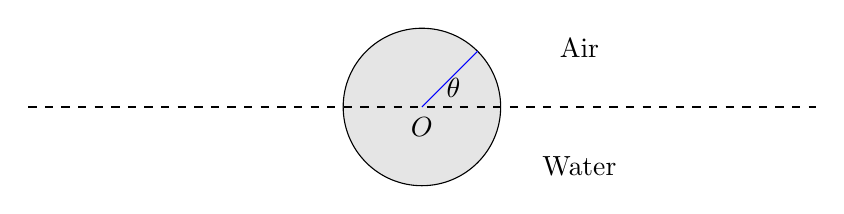
\begin{tikzpicture}
 \draw[solid, fill=gray!20] (0, 0) circle (1cm);
  \draw [color=blue!150](0,0) -- (1/2^0.5,1/2^0.5);
\coordinate[label = $\theta$] () at (0.4, 0);
\coordinate[label = $O$] (O) at (0, -0.5);
\coordinate[label = Air] () at (2, 0.5);
\coordinate[label = Water] () at (2, -1);
\draw[dashed] (-5,0) -- (5,0);
 \end{tikzpicture}

\begin{equation}\label{hotpotfloat}
\left\{
\begin{array}{ll}
u_t=D\Delta u,& \textbf{x}\in B_0(R),t\in\mathbb R^+,\\
u(\textbf{x},0)=25 \text{\textdegree{C}},&\textbf{x}\in B_0(R),\\
u(\textbf{x},t)=\left\{
\begin{array}{ll}
25 \text{\textdegree{C}},& \theta\in (0,\pi),\\
100 \text{\textdegree{C}},& \theta\in (-\pi,0),
\end{array}
\right.
\end{array}
\right.
\end{equation}
where we applied the polar coordinates with $u(\textbf{x},t)=u(r,\phi,\theta,t)$, $r\in(0,R)$, $\phi\in(0,2\pi)$, $\theta\in(-\pi,\pi)$.  If the ball is not half dipped into the water, then a generalization of the surface separation is needed to characterize the BC and I leave it to motivated students.  Indeed, we also do not consider the surface oil (layer) which might have different influence on the cooking from the boiling water.
\end{solution}





\item Let us revisit the following problem in HW 4: let $f(x)$ be a function with a jump at $x=0$ defined over $(-\pi,\pi)$ as: $f(x)=1$ for $x\in[0,\pi)$ and $f(x)=-1$ for $x\in(-\pi,0)$.  First of all, we know $f(x)$ can be written into series as
       \begin{equation}\label{limit}
f(x)=\sum_{n=1}^\infty C_n\sin nx.
 \end{equation}
   Now let us approximate it by the sum of first $N$ terms as before
   \begin{equation}\label{cauchy}
 f_N(x):=\sum_{n=1}^N C_n\sin nx
 \end{equation}
    for some large $N$.  Plot $f_N(x)$ over $(-\pi,\pi)$ for $N=2,4,8,16$ on the same graph.  Try $N=16,32$ and $64$ again.  What are your observations?  You can try with even larger $N$s.
    \begin{solution}
Note that $C_n=\frac{2}{n}(1-(-1)^n)$ in (\ref{cauchy}).  The plots in Figure \ref{figure55a} are recovered from a previous HW.
     \begin{figure}[h!]\vspace{-8mm}
  \centering
\includegraphics[width=0.9\textwidth]{hw3figure9.eps}
\caption{Finite sum $f^N$ and oscillations for $N$ large.  We observe the non-convergence (in pointwise sense) of $f^N$ for $N$ large, though the error converges to zero in $L^2$.  Again this is because its limit is merely $L^2$, but not continuous, hence pointwise convergence is not expected.}\label{figure55a}
\end{figure}
    \end{solution}


\item We recall from baby calculus that a number sequence is called a Cauchy sequence if $|a_{n+1}-a_n|$ is arbitrarily small if $n$ is arbitrarily large; for example $a_n=\frac{1}{n}$ is Cauchy because $|a_{m}-a_{n}|=\frac{m-n}{mn}<\frac{1}{n}\rightarrow 0$ as $n\rightarrow \infty$.  And a region is called \textbf{complete} if every Cauchy converges in it.  For example, $(0,1)$ is not closed since $a_n=\frac{1}{n}$ is Cauchy but $a_n\rightarrow 0\not\in (0,1)$, while $[0,1]$ is closed.  There are more or less rigourous definitions of a closed region.  We have a cousin of closedness when it comes to function space, i.e., the completeness.  For a function space $\mathcal X$ endowed with a norm (called a normed space or a metric space) denoted by $\Vert \cdot \Vert_{\mathcal X}$, we say that a function sequence is Cauchy if $\Vert f_{n+1}(x)-f_n(x) \Vert_{\mathcal X}\rightarrow 0$ as $n\rightarrow \infty$.  Here the only difference/generalization is that the absolute value distance is replaced by the so-called ``norm"; then we say that space $\mathcal X$ is \textbf{complete} if every Cauchy sequence converges (in the space or that norm).  For instance, one can prove that $L^p(\Omega)$, $p\in(1,\infty)$ is complete (well, you should have learned in your Analysis course or learn it by yourself otherwise); moreover, in Euclidean space complete is equivalent as closed and bounded.

Going back to the completeness of $L^p$, if $f_n$ is Cauchy in $L^p$ its limit must be in $L^p$.  Then one usually needs to verify the Cauchy-ness of the sequences.

i) prove that the sequence $f_N$ given by (\ref{cauchy}) is Cauchy in $L^2$.  Then according to i), its limit (\ref{limit}) belongs to $L^2$ and this gives you proof of the convergence fashion we had in class, at least for this particular example;

ii) plot $\Vert f_{n+1} -f_n \Vert_{L^2((-\pi,\pi))}$ for $n=1,2,...$ and you should observe the convergence; indeed, to better illustrating the convergence it makes sense to plot the log error $\mathcal E_n:=\log (\Vert f_{n+1} -f_n \Vert_{L^2})$ for $n$ large, for instance starting from $10$.  Remark: MATLAB can evaluate the integrals hence you do not have to do it by brutal force;

iii) try different $L^p$ norms with $p=5,10,20,30$,... and do the same as in ii); plot them in the same graph; what are your observations?

iv) now find the $\max$-norm and do the same as in ii).

\begin{solution}
The verification of Cauchyness is rather straightforward and I skip the calculations here.
\begin{figure}[h!]\vspace{-3mm}
\begin{minipage}{0.5\columnwidth}
\includegraphics[width=1\columnwidth,height=35mm]{hw4figure32.eps}
\caption*{Absolute errors in $L^2$}
\end{minipage}
\begin{minipage}{0.5\columnwidth}
\includegraphics[width=1\columnwidth,height=35mm]{hw4figure31.eps}
\caption*{Absolute errors in $L^p$}
\end{minipage}
\vspace{-1mm}\caption{ }\label{ }
\end{figure}

\begin{figure}[h!]\vspace{-3mm}
\begin{minipage}{0.5\columnwidth}
\includegraphics[width=1\columnwidth,height=35mm]{hw4figure322.eps}
\caption*{Log errors in $L^p$ for different $p$}
\end{minipage}
\begin{minipage}{0.5\columnwidth}
\includegraphics[width=1\columnwidth,height=35mm]{hw4figure33.eps}
\caption*{Errors in $L^\infty$ and log errors}
\end{minipage}
\vspace{-1mm}\caption{For each $p$ one observes the oscillating dissipation of errors.  It seems that an exponential decay is not expected.}
\end{figure}
\end{solution}


\end{enumerate}


\end{document}
\endinput
